\chapter{PRIMJER IMPLEMENTACIJE DPIV KROS-KORELACIJE U MATLAB-u}
\label{chap:Poglavlje6}
U ovom poglavlju dan je jednostavan primjer funkcioniranja DPIV kros-korelacije u MATLAB programskom jeziku. Za početak ponovno je ukratko opisana (normalizirana) kros-korelacije radi lakšeg razumijevanja u MATLAB implementirane funkcije \textit{normxcorr2} koja računa normaliziranu 2D kros-korelaciju.
\section{Koncept podudaranja predloška sa slikom koristeći kros-korelaciju}
\label{podudaranjePredlSlika}
Jedan od glavnih zadataka i ideje upotrebe normalizirane 2D kros-korelacije je detekcija značajki slika (signala). Drugim riječima prepoznavanje obilježja predloška na drugoj većoj slici, to jest pronalazak lokacije gdje se predložak poklapa sa većom slikom. Primjer predloška i slike na kojoj je potrebno pronaći zadani predložak prikazan je na \textit{Slici \ref{sl:6.1}}
\begin{figure}[h]  
	\centering
	%\usepackage{graphicx}
	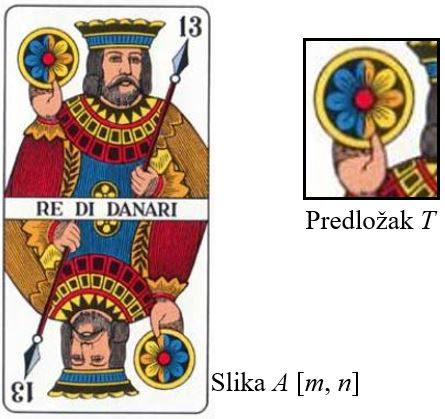
\includegraphics[width=7cm]{./6_PrimjerKrosKorelacije/slika6_1.jpg} 
	\caption{Primjer mogućeg lociranja predloška $T$ na slici $A$}
	\label{sl:6.1}
\end{figure}
\par
Mogući način rješenja problema je da se predložak $T$ "pusti da klizi" po većoj slici $A$, te dalje na svakoj poziciji slike $A$ i predloška $T$ bi se izračunala razlika između predloška i slike (u području preklapanja). Na taj način bi se dobila matrica vrijednosti razlika između predloška i slike, te na mjestu gdje je vrijednost matrice najmanja, najveća je vjerojatnost da je to pozicija predloška. Matematička formulacija opisanog rješenja može biti opisana uz pomoć minimiziranja kvadrata Euklidove duljine (ekvivalentno duljini između dvije točke):
\begin{equation}
	E[i,\, j] = \sum_{m}\sum_{n}\left(A[m,\, n]-T[m-i,\, n-j]\right)^{2}
	\label{eqn:6.1}
\end{equation}
gdje je $A$ slika veličine $[m,\, n]$, a $T$ predložak koji sadrži neku značajku slike $A$ trenutno pozicioniran na lokaciji $i,\, j$. Ako je jednadžba \ref{eqn:6.1} jednaka nuli jasno je kako je pronađena lokacija gdje predložak točno odgovara $i,\, j$ mjestu na slici. Kvadriranjem izraza \ref{eqn:6.1} dobije se:
\begin{equation}
	E[i,\, j] = \sum_{m}\sum_{n}\left(A^{2}[m,\, n]+T^{2}[m-i,\, n-j]-2A[m,\, n]T[m-i,\, n-j]\right)
	\label{eqn:6.2}
\end{equation}
Iz izraza je vidljivo kako je minimiziranje desne strane jednadžbe \ref{eqn:6.1} ekvivalentno maksimiziranju posljednjeg člana iz jednadžbe \ref{eqn:6.2}. Drugim riječima posljednji član (kros-korelacija) jednadžbe \ref{eqn:6.2}  predstavlja mjeru sličnosti između slike $A$ i predloška $T$.
\begin{equation}
	\boxed{R[i,\, j]=\underbrace{\sum_{m}\sum_{n}A[m,\, n]\, T[m-i,\, n-j] = \boldsymbol{T}\otimes \boldsymbol{A}}_{\text{2D kros-korelacija}}}
	\label{eqn:6.3}
\end{equation}
Korištenje izraza \ref{eqn:6.3} kod podudaranja predložaka treba dodatno biti modificirano iz sljedećeg razloga. Za slučaj da "energija" slike $\sum\sum A^{2}(m,\, n)$ varira sa pozicijom, podudaranje koristeći izraz \ref{eqn:6.3} će biti pogrešno. Razlog je u tome što prilikom množenja predloška sa dijelovima slike u kojima predložak ne pripada, može se dogoditi da su vrijednosti slike u tim dijelovima automatski veće nego u dijelu gdje predložak pripada (npr. zbog toga što je u tim dijelovima intenzitet svijetla veći). Tako pomnožene vrijednosti daju u startu veće korelacijske iznose te korištenje kros-korelacije u takvim trenucima nema efekta. Rješenje ovom problemu leži u normalizaciji izraza \ref{eqn:6.3} kojim će se sve automatski velike vrijednosti dovesti na istu razinu u svim područjima slike, tj. energetske razlike unutar slike biti će "ispeglane":
\begin{equation}
	\boxed{N[i,\, j]=\underbrace{\dfrac{\sum_{m}\sum_{n}A[m,\, n]\,T[m-i,\, n-j]}{\sqrt{\sum_{m}\sum_{n}A^{2}[m,\, n]}\sqrt{\sum_{m}\sum_{n}T^{2}[m-i,\, n-j]}}}_{\text{Normalizirana 2D kros-korelacija}}}
	\label{eqn:6.4}
\end{equation}
Lijevi član u nazivniku $\sqrt{\sum_{m}\sum_{n}A^{2}[m,\, n]}$ predstavlja "energiju" slike $A$ u području gdje se slika trenutno preklapa sa predloškom $T$, dok desni član $\sqrt{\sum_{m}\sum_{n}T^{2}[m-i,\, n-j]}$ predstavlja energiju predloška. Na ovaj način kros-korelacija postaje neosjetljiva ne promjene intenziteta slike. \\
U sklopu ovog rada radi lakšeg shvaćanja kros-korelacije u MATLAB-u je odrađen jednostavan primjer pronalaska predloška na slici (primjer sa \textit{Slike \ref{sl:6.1}}) U primjeru je korištena funkcija \textit{normxcorr2} koja prihvaća dva argumenta: prvi argument je predložak, a drugi slika koja će se pretraživati. Oba argumenta moraju biti učitana u obliku slike u sivom tonu. Za slučaj da učitane slike nisu sivom tonu, pozivanjem funkcije \textit{im2gray} slika se prebacuje iz RGB modela boje u sivi ton. Nakon izvršavanja kros-korelacijske funkcije, dobije se korelacijska matrica kojoj je onda potrebno pronaći najveću vrijednost koja u konačnici označava i središte lokacije predloška na slici. MATLAB kod dostupan je u \textit{Prilogu \ref{prilog}1}.
\FloatBarrier
\section{Primjer DPIV kros-korelacije u MATLAB-u}
\label{PIVkod}
U sklopu rada napravljen je i pokazni jednostavni DPIV kros-korelacijski primjer koda (\textit{Prilog \ref{prilog}2}) u svrhu jasnijeg razumijevanja digitalne PIV evaluacije. Za početak učitane su dvije uzastopne PIV snimke, koje su također odmah prebačene u sivi spektar (u ovom primjeru učitane su sintetičke snimke koje su generirane u PIVlab softveru prema postavkama prikazanim na \textit{Slici \ref{sl:6.2}}).
\begin{figure}[h]  
	\centering
	%\usepackage{graphicx}
	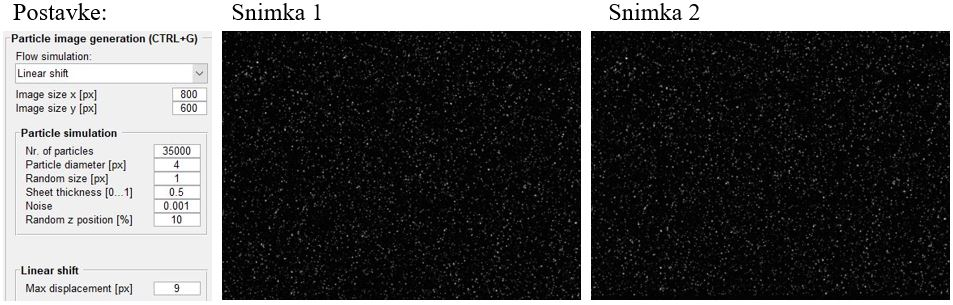
\includegraphics[width=16cm]{./6_PrimjerKrosKorelacije/slika6_2.jpg} 
	\caption{Postavke generiranih snimki u PIVlab-u, kao tip strujanja odabran je linearni pomak prema gore sa maksimalnom vrijednosti pomaka u iznosu od 9 pixela}
	\label{sl:6.2}
\end{figure}
\par
Nakon učitavanja slika u programu je kreirana matrica koja definira prozor ispitivanja, te je odabrana standardna veličina od $64\times 64$ pixela. Naime, kao što je već u ranijim poglavljima objašnjeno, kod PIV kros-korelacije se koristi tzv. strategija podijeli i vladaj (\textit{eng. divide and rule}), prema kojoj se cijela snimka podijeli na mrežu prozora ispitivanja, te se za svaki prozor ispitivanja određuje prosječna brzina svih čestica unutar istoga. Iz toga je jasno kako rezolucija polja brzina ovisi o veličini samog prozora ispitivanja. Da se kreira mreža u programu je još definiran odmak od rubova snimke kojim se osigurava da prozor ispitivanja ne kreće iz ishodišta snimke. Na \textit{Slici \ref{sl:6.3}} grafički su nacrtane dvije uzastopne PIV snimke. Na snimci 1 jasno se vidi odabrani princip generiranja mreže, te treba napomenuti kako mreža u ovom kodu nije centrirana u sredini snimke (pošto nema utjecaja na rješenje), pa razmak između lijeve i desne, odnosno gornje i donje strane nije isti. Čestice na snimci 2 ponovno su pravocrtno pomaknute prema gore.
\begin{figure}[h]  
	\centering
	%\usepackage{graphicx}
	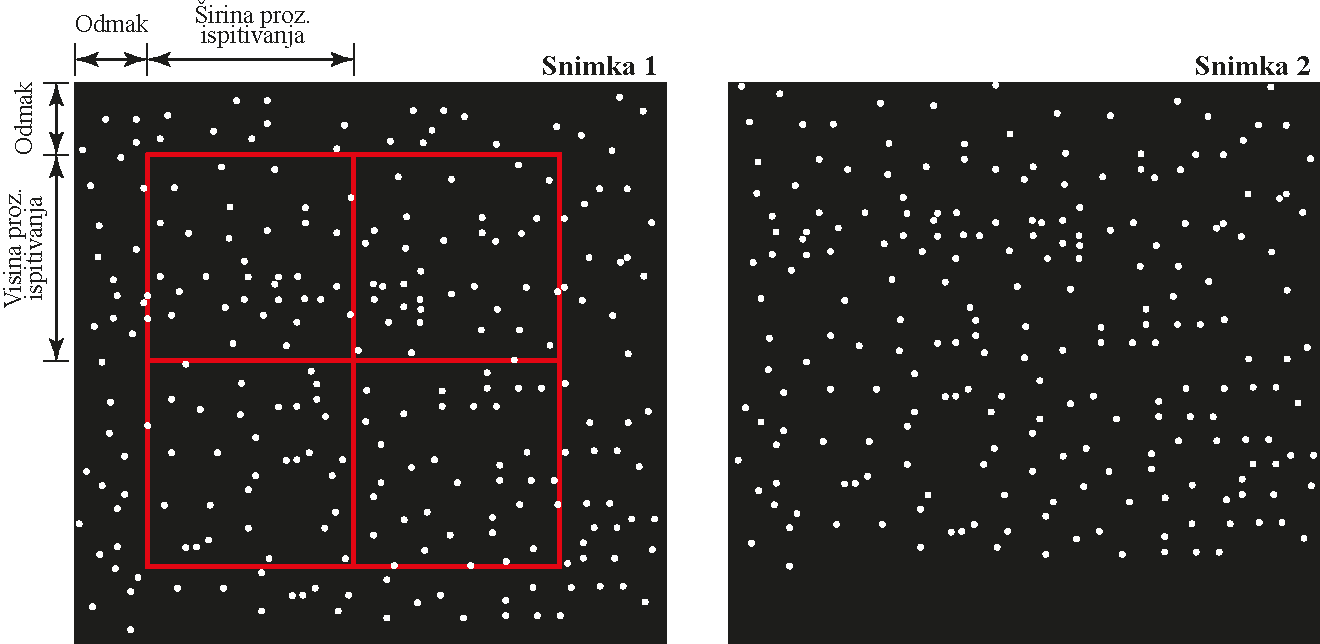
\includegraphics[width=13.5cm]{./6_PrimjerKrosKorelacije/slika6_3.pdf} 
	\caption{Grafički prikaz generiranje mreže koja opisuje prozore ispitivanja, u ovom slučaju postoje 4 prozora}
	\label{sl:6.3}
\end{figure}
\par
Nakon generiranja mreže sljedeći korak je pojedinačna korelacijska analiza svakog prozora ispitivanja posebno. Kros-korelacija se odvija u ugniježđenoj \textit{for} petlji koja se "vrti" ovisno o broju prozora ispitivanja. Laički, sada je cilj pronaći lokaciju manjeg prozora ispitivanja sa snimke 1 na snimci 2, na isti princip kao i u prethodnom poglavlju. U ovom kodu jedina razlika u odnosu na prethodni kod u pretraživanju je ta da se predložak (prozor ispitivanja iz snimke 1) neće pretraživati po cijeloj domeni snimke 2, nego samo u dijelu koji je malo veći od prozora ispitivanja (\textit{Slika \ref{sl:6.4}}). Razlog je u tome što kod PIV mjerenja postoji određena ideja gdje se nalazi predložak na sljedećoj slici, pa bi pretraživanje cijele domene bilo neefikasno. 
\begin{figure}[h]  
	\centering
	%\usepackage{graphicx}
	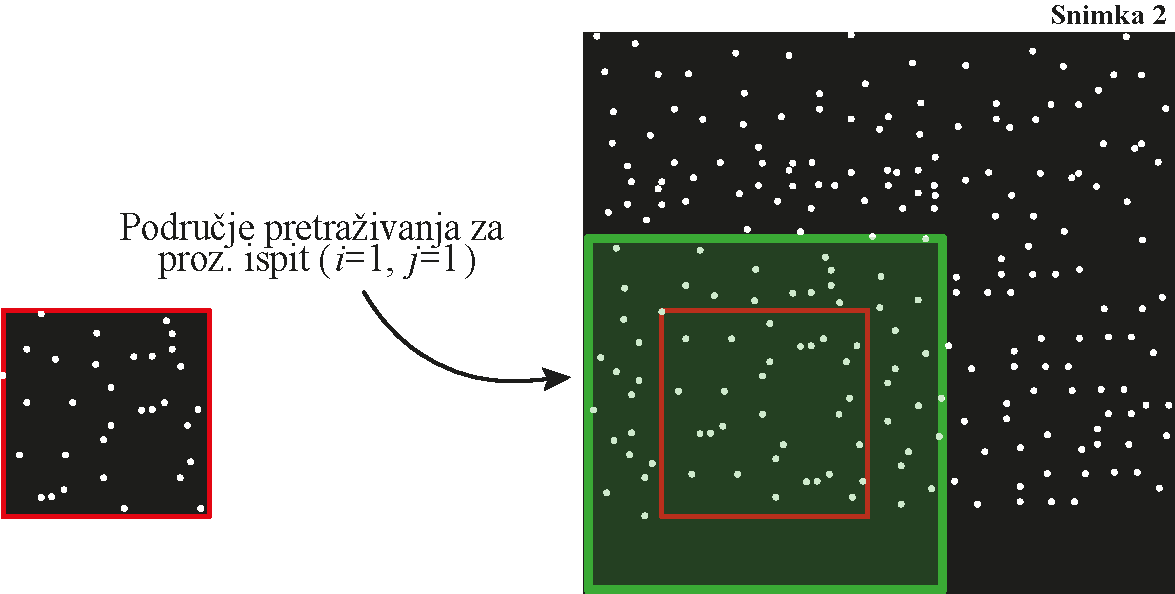
\includegraphics[width=13cm]{./6_PrimjerKrosKorelacije/slika6_4.pdf} 
	\caption{Grafički prikaz područja pretraživanja za prozor ispitivanja $(i=1,\, j=1)$}
	\label{sl:6.4}
\end{figure}
\par
Odabir veličine područja pretraživanja na snimci 2 obično se uzima da bude 2 puta veća od prozora ispitivanja, ali ipak veličina ovisi o parametrima mjerenja, te u skladu s njima mora biti podešena. Za prvu iteraciju \textit{for} petlje područje ispitivanja sa \textit{Slike \ref{sl:6.4}} je ulazni argument u obliku predloška, dok je područje pretraživanja ulazni argument za sliku funkcije \textit{normxcorr2}. Nakon što su slike korelirane, dobije se matrica u kojoj se pronađe najveća vrijednost korelacije, te se koordinate privremeno pohrane da bi se iz njih izračunao pomak koje je jednak razlici koordinata najveće vrijednosti korelacije i koordinatama mjesta prozora ispitivanja. U ovom slučaju postoji samo pomak u y-smjeru (prema gore) kako je prikazano i na \textit{Slici \ref{sl:6.5}}. Sljedeći korak analize je iteracija kroz sve generirane prozore ispitivanja dok se konačno ne dobiju matrice x i y pomaka za sve prozore.
\begin{figure}[h]  
	\centering
	%\usepackage{graphicx}
	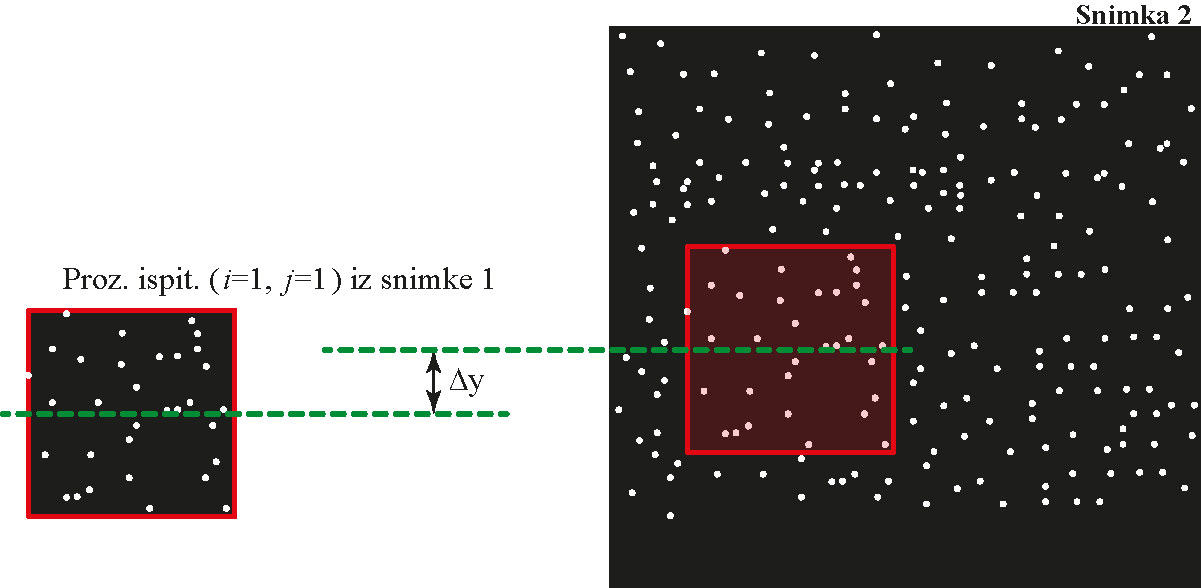
\includegraphics[width=13cm]{./6_PrimjerKrosKorelacije/slika6_5.pdf} 
	\caption{Grafički prikaz dobivenog pomaka}
	\label{sl:6.5}
\end{figure}
\par
Na sljedećim slikama prikazano je nekoliko primjera u kodu izračunanih polja brzina. Na \textit{Slici \ref{sl:6.6}} prikazan je rezultat analize snimki sa \textit{Slike \ref{sl:6.1}}. Na lijevoj slici vidi se primjer analiziran u MATLAB kodu, dok desna slika prikaziva rezultat istih snimki koji je analiziran u PIVlab-u. Kros-korelacija na analiziranoj snimci ispravno je izračunala polje pomaka kod obje analize, te je prosječni iznos svih pomaka 9 pixela, baš kako je i zadano pri generiranju sintetičkih snimki. Iz slika je zanimljivo vidjeti kako PIVlab i na default-nim postavkama pretprocesira analizirane snimke, te pojača kontrast i u suštini pripremi snimke za što kvalitetniju kros-korelacijsku analizu.
\begin{figure}[h]  
	\centering
	%\usepackage{graphicx}
	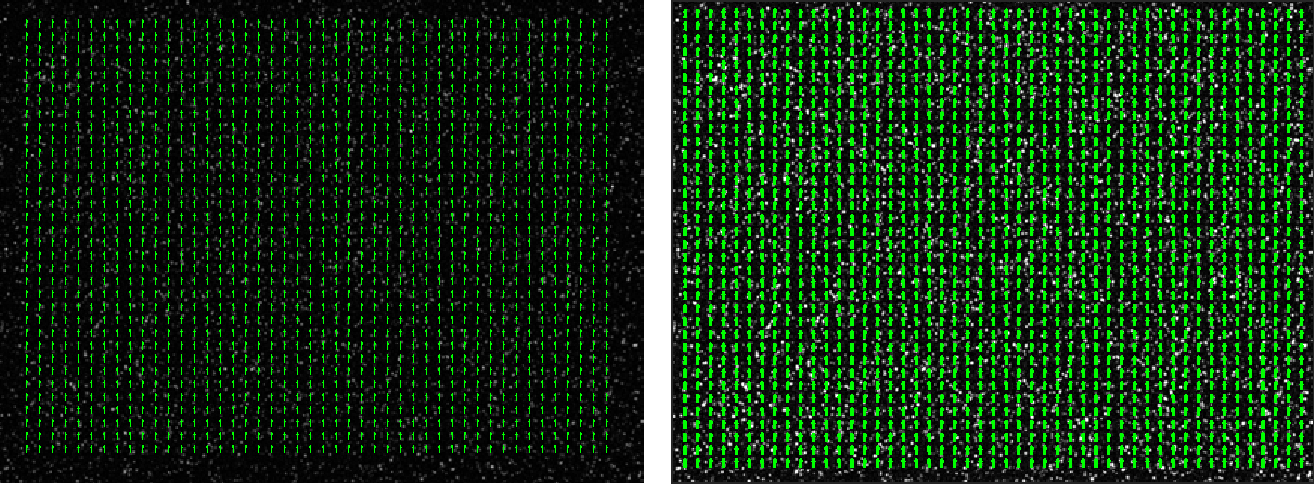
\includegraphics[width=15.5cm]{./6_PrimjerKrosKorelacije/pravocrtnoKodlivoPIVlabdesno.pdf} 
	\caption{Rezultat DPIV kros-korelacije pravocrtnog pomaka čestica u kodu (lijevo) i PIVlab softveru (desno)}
	\label{sl:6.6}
\end{figure}
\par
Na \textit{Slici \ref{sl:6.7}} prikazana je analiza dva Rankine vrtloga \cite{wiki:Rankine} također umjetno generirana u PIVlab softveru. Na slikama je vidljivo kako napisani program već kod malo složenijih strujanja i manje informacijski kvalitetnih snimki daje nepravilne vektore. Dok PIVlab softver uz svoju robusnu pretprocesorsku analizu odlično opisuje polje pomaka dva vrtloga.
\begin{figure}[h]  
	\centering
	%\usepackage{graphicx}
	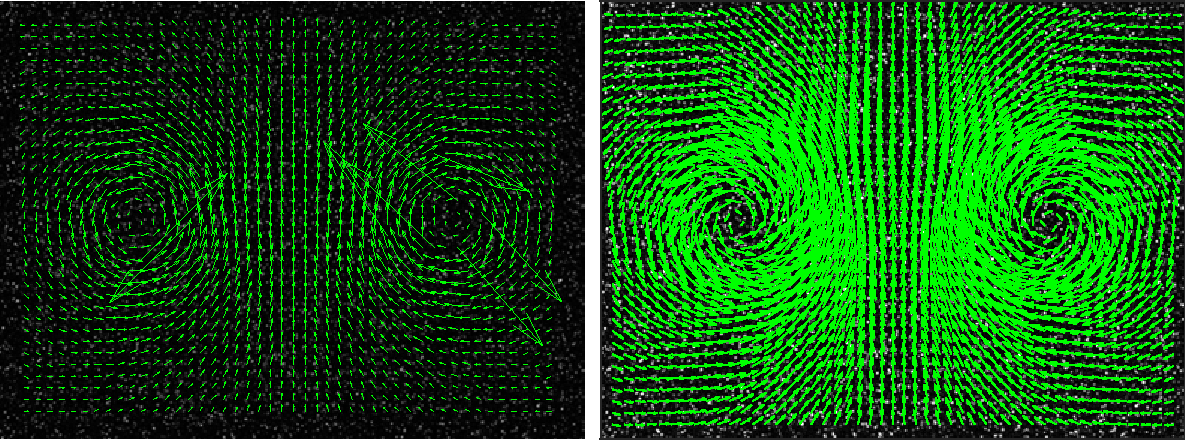
\includegraphics[width=15.5cm]{./6_PrimjerKrosKorelacije/vortexKodlivoPIVlabdesno.pdf} 
	\caption{Rezultat DPIV kros-korelacije dva Rankine vrtloga u kodu (lijevo) i PIVlab softveru (desno)}
	\label{sl:6.7}
\end{figure}